\documentclass[a4paper,12pt,oneside,onecolumn,final,fleqn]{repUERJ}
% ---
% Pacotes fundamentais 
% ---
\usepackage[english,brazil]{babel}  % adequação para o português Brasil
\usepackage[utf8]{inputenc} % Determina a codificação utilizada
                            % (conversão automática dos acentos)
\usepackage{makeidx}        % Cria o índice
\usepackage{hyperref}       % Controla a formação do índice
\usepackage{indentfirst}    % Indenta o primeiro paragrafo de
                            % cada seção.
\usepackage{graphicx}       % Inclusão de gráficos
\usepackage{subfig}
\usepackage{amsmath}        % pacote matemático
\usepackage{bm}             % pacote de fontes matemáticas
\usepackage{lscape}         % pacote para colocar páginas em modo paisagem
\usepackage{array}


% ---
% Pacote auxiliar para as normas da UERJ
% ---
\usepackage[frame=no,font=default]{repUERJformat}
\usepackage[line=yes]{repUERJpseudocode}
% ---
% Pacotes de citacoes
% ---
\usepackage[alf,abnt-repeated-author-omit=no]{abntex2cite}


\selectlanguage{brazil} % setando o idioma global para português



% ********************************************************************
% ********************************************************************
% Área Reservada para incluir os novos comandos
% ********************************************************************
% ********************************************************************

% Comandos de comentários
\definecolor{green}{rgb}{0.1, 0.4, 0.1}
\newcommand\red[1]{{\color{red}#1}}
\newcommand\sred[1]{{\color{red}\uline{#1}}}
\newcommand\blue[1]{{\color{blue}#1}}
\newcommand\sblue[1]{{\color{blue}\uline{#1}}}
\newcommand\green[1]{{\color{green}#1}}
\newcommand\sgreen[1]{{\color{green}\uline{#1}}}
\newcommand\orange[1]{{\color{orange}#1}}
\newcommand\sorange[1]{{\color{orange}\uline{#1}}}
%o comando \sout funciona para riscar o texto

% Abaixo tem-se alguns exemplos de definição de comandos

\newcommand\dd{\mathrm{d}} % d de derivada
\newcommand\DD{\mathrm{D}} % D de derivada
\newcommand\ee{\mathrm{e}} % número natural: e
\newcommand\ii{\mathrm{i}} % número complexo: i

\newcommand\Vol{\mathcal{V}} % Simbolo de volume

\newcommand\Vector[1]{\mbox{\boldmath$#1$}} % comando para colocar vetores
\newcommand\Tensor[1]{\mbox{\boldmath$\mathrm{#1}$}} % comando para colocar tensores/matrizes

%Alguns exemplos de definição de vetores, tensores e matrizes
\newcommand\vvec{\Vector{v}} % vetor
\newcommand\Tten{\Tensor{T}} % Tensor
\newcommand\Mmat{\Tensor{M}} % Matriz

% Alguns parâmetros adimensionais
\newcommand\Bi{\mathrm{Bi}} % Número de Biot
\newcommand\Rey{\mathrm{Re}} % Número de Reynolds
\newcommand\Ma{\mathrm{Ma}} % Número de Mach
\newcommand\Pe{\mathrm{Pe}} % Número de Péclet

\newcommand\Dh{D_H} % Diâmetro hidráulico

% Alguns índices máximos 
\newcommand\nmax{n_{\text{max}}}
\newcommand\mmax{m_{\text{max}}}
\newcommand\imax{i_{\text{max}}}
\newcommand\jmax{j_{\text{max}}}








% ********************************************************************
% ********************************************************************
% Informações de autoria e institucionais
% ********************************************************************
% ********************************************************************

%---------------------------------------------------------------------
% Imagens pretextuais (precisam estar no mesmo diretório deste arquivo .tex)
%---------------------------------------------------------------------

\logo{logo_uerj_cinza.png}
\marcadagua{marcadagua_uerj_cinza.png}{1}{160}{255}

%---------------------------------------------------------------------
% Informações da instituição
%---------------------------------------------------------------------
\instituicao{Universidade do Estado do Rio de Janeiro}  %Universidade
            {Centro de Tecnologia e Ciências}  %Centro
            {Faculdade de Ciências da Computação} %Unidade
            {Departamento de Computação} %Departamento

%---------------------------------------------------------------------
% Informações da autoria do documento
%---------------------------------------------------------------------

\autor{Felipe}
      {Ferme Cajueiro}
      {F. F. C.} % iniciais do nome

\titulo{O uso de Frameworks no desenvolvimento de Sistema para Gerenciamento de Clientes e Ordens de Serviços} %Título do trabalho acadêmico em português
\title{The use of Frameworks in the Development of a Customer and Service Order Management System} %Título do trabalho acadêmico em inglês





\orientador{Prof. Adriana Aparicio Sicsú Ayres do Nascimento} %cargo, ex.: Prof., Profa., Eng. , etc...
		   %{Daniel}{José Nahid Mansur Chalhub, DSc} %Nome sobrenome com a titulação ao final. Exemplo: D.Sc., Ph.D., M.Sc., B.Sc., etc.
           %{Universidade do Estado do Rio de Janeiro (UERJ) - DEPCOMP-COMP} % Instituição e Departamento ou PPG


%Opcional, Comente as linhas de coorientador caso não tenha
%\coorientador{cargo}  %cargo, ex.: Prof., Profa., Eng. , etc...
           %{nome}{sobrenome, titulação}  %Nome sobrenome com a titulação ao final. Exemplo: D.Sc., Ph.D., M.Sc., B.Sc., etc.
           %{unidade -- instituição} % Departamento ou PPG e Instituição 

%---------------------------------------------------------------------
% Grau pretendido (Doutor, Mestre, Bacharel, Licenciado) e Curso
%---------------------------------------------------------------------
%Descomente as sua opções

\newcommand\artigo{à}%Projeto de graduação
%\newcommand\artigo{ao}%Pós Graduação


\grau{Graduação}
%\grau{Mestre} 
%\grau{Doutor}


\curso{Ciências da Computação}
\newcommand\grauTitulo{Bacharel em Ciências da Computação}  


\areadeconcentracao{APIs} %Projeto de Graduação
%\areadeconcentracao{Fenômenos de Transporte} %Pós Graduação
%\areadeconcentracao{Mecânica dos Sólidos} %Pós Graduação



%---------------------------------------------------------------------
% Informações adicionais (local, data e paginas)
%---------------------------------------------------------------------

\local{Rio de Janeiro} 
\data{16}{Maio}{2024} % Exemplo: \data{21}{Março}{2016}

% ********************************************************************
% ********************************************************************
% Configurações de aparência do PDF final
% ********************************************************************
% ********************************************************************

% alterando o aspecto da cor azul
\definecolor{blue}{RGB}{41,5,195}
%\definecolor{apricot}{RGB}{251,206,177}

% informações do PDF
\hypersetup{
  unicode=false,
  pdftitle={\UERJtitulo},
  pdfauthor={\UERJautor},
  pdfsubject={\UERJpreambulo},
  pdfkeywords={PALAVRAS}{CHAVES}{\chaveA}{\chaveB}{\chaveC}{\chaveD},
  pdfproducer={\packagename}, % producer of the document
  pdfcreator={\UERJautor},
  colorlinks=true,            % false: boxed links; true: colored links
  linkcolor=black,            % color of internal links blue
  citecolor=black,            % color of links to bibliography blue
  filecolor=black,            % color of file links magenta
  urlcolor=black,
  bookmarksdepth=4,
  %backref=true,
  %pagebackref=true,
  %bookmarks=true,
}

% ********************************************************************
% ********************************************************************
% Início do documento
% ********************************************************************
% ********************************************************************
% ---
% compila o índice; se não for usar, comentar
% ---
\makeindex
% ********************************************************************
% ********************************************************************
\begin{document}
% ----------------------------------------------------------
%% ELEMENTOS PRE-TEXTUAIS
% ----------------------------------------------------------
\frontmatter
% ----------------------------------------------------------
% Capa e a folha de rosto
% ----------------------------------------------------------
\capa
\folhaderosto
% ----------------------------------------------------------
% Inserir a ficha catalográfica
% ----------------------------------------------------------
% ---
% A biblioteca deverá providenciar a ficha catalográfica. Salve a ficha no
% formato PDF. Use o nome do arquivo PDF como argumento do comando. 
% Exemplo: ficha catalográfica é o arquivo 'Ficha.pdf' na pasta "B.PreTextual"
%     \fichacatalografica{B.PreTextual/Ficha.pdf}
%
% Enquanto não possuir a ficha catalográfica, use o comando sem argumentos.
% ---
\fichacatalografica{B.PreTextual/Ficha.pdf}



% ----------------------------------------------------------
% Folha de aprovação
% ----------------------------------------------------------

%Após obter a assinatura dos membros da banca, comente as linhas a baixos e insira o pdf com as assinaturas na pasta "B.PreTextual"


% Ajustar o espaço entre as assinaturas abaixo
\newcommand{\spc}{0.25cm}

\begin{folhadeaprovacao}
	\vspace{\spc} % Espaço entre assinaturas
	\assinatura{Professor numero 2}{Universidade do Estado do Rio de Janeiro (UERJ)} %Exemplo
	\vspace{\spc} % Espaço entre assinaturas
	\assinatura{Professor numero 3}{Universidade do Estado do Rio de Janeiro (UERJ)}
	\vspace{\spc} % Espaço entre assinaturas
	\assinatura{Professor numero 4}{Universidade do Estado do Rio de Janeiro (UERJ)}
	\vspace{\spc} % Espaço entre assinaturas
	\assinatura{Professor numero 5}{Universidade do Estado do Rio de Janeiro (UERJ)}
\end{folhadeaprovacao}


% Após colocar o pdf com as assinaturas na pasta "B.PreTextual", comente todo o ambiente "folhadeaprovacao" acima, descomente a linha abaixo e insira o nome correto do arquivo pdf:
%\includepdf[pages=1]{B.PreTextual/ficha.pdf} %exemplo


% ----------------------------------------------------------
% Dedicatória
\pretextualchapter{Dedicatória}
\vfill
Eu dedico essa tese para uma pessoa muito especial.






% ----------------------------------------------------------
% Agradecimentos
\pretextualchapter{Agradecimentos}
Agradeço aos amigos que fiz na faculdade que sempre estiveram ao meu lado, oferecendo seu apoio incondicional e amizade sincera. Em momentos difíceis, eles foram minha âncora, lembrando-me do valor da persistência e da força que reside em mim mesmo.



% ----------------------------------------------------------
% Epigrafe (opcional)
\pretextualchapter{}
\vfill
\begin{flushright}
	Feliz, feliz, feliz... Estou tão feliz\\
	\textit{Uma criança feliz}
\end{flushright}










% ----------------------------------------------------------
%% RESUMO
% se não for usar a quarta palavra chave, deixar o campo vazio: {}
\palavraschaves{primeira palavra chave}
{segunda palavra chave}
{terceira palavra chave}
{quarta palavra chave (se houver)}



\pretextualchapter{Resumo}
\referencia % linha em branco depois

Lorem ipsum dolor sit amet, consectetur adipiscing elit, sed do eiusmod tempor incididunt ut labore et dolore magna aliqua. Ut enim ad minim veniam, quis nostrud exercitation ullamco laboris nisi ut aliquip ex ea commodo consequat. Duis aute irure dolor in reprehenderit in voluptate velit esse cillum dolore eu fugiat nulla pariatur. Excepteur sint occaecat cupidatat non proident, sunt in culpa qui officia deserunt mollit anim id est laborum. Sed ut perspiciatis unde omnis iste natus error sit voluptatem accusantium doloremque laudantium, totam rem aperiam, eaque ipsa quae ab illo inventore veritatis et quasi architecto beatae vitae dicta sunt explicabo. Nemo enim ipsam voluptatem quia voluptas sit aspernatur aut odit aut fugit, sed quia consequuntur magni dolores eos qui ratione voluptatem sequi nesciunt. Neque porro quisquam est, qui dolorem ipsum quia dolor sit amet, consectetur, adipisci velit, sed quia non numquam eius modi tempora incidunt ut labore et dolore magnam aliquam quaerat voluptatem. Ut enim ad minima veniam, quis nostrum exercitationem ullam corporis suscipit laboriosam, nisi ut aliquid ex ea commodi consequatur? Quis autem vel eum iure reprehenderit qui in ea voluptate velit esse quam nihil molestiae consequatur, vel illum qui dolorem eum fugiat quo voluptas nulla pariatur?

 xxxxxxxxxxxxxxxxxxxxxxxxxxxx xxxxxxxxxxxxxxxx teste de hiphenização: monumental bla bla bla\\

\imprimirchaves % linha em branco antes




% ----------------------------------------------------------
% Abstract
\begin{otherlanguage}{english}
  \keywords{first keyword}
{second keyword}
{third keyword}
{fourth keyword (if any)}


\pretextualchapter{Abstract}
\reference % linha em branco depois

% O resumo em inglês deve ser organizado em apenas um parágrafo mesmo.

 Happiness deserves a English description. Lorem ipsum dolor sit amet, consectetur adipiscing elit, sed do eiusmod tempor incididunt ut labore et dolore magna aliqua. Ut enim ad minim veniam, quis nostrud exercitation ullamco laboris nisi ut aliquip ex ea commodo consequat. Duis aute irure dolor in reprehenderit in voluptate velit esse cillum dolore eu fugiat nulla pariatur. Excepteur sint occaecat cupidatat non proident, sunt in culpa qui officia deserunt mollit anim id est laborum. Sed ut perspiciatis unde omnis iste natus error sit voluptatem accusantium doloremque laudantium, totam rem aperiam, eaque ipsa quae ab illo inventore veritatis et quasi architecto beatae vitae dicta sunt explicabo. Nemo enim ipsam voluptatem quia voluptas sit aspernatur aut odit aut fugit, sed quia consequuntur magni dolores eos qui ratione voluptatem sequi nesciunt. Neque porro quisquam est, qui dolorem ipsum quia dolor sit amet, consectetur, adipisci velit, sed quia non numquam eius modi tempora incidunt ut labore et dolore magnam aliquam quaerat voluptatem. Ut enim ad minima veniam, quis nostrum exercitationem ullam corporis suscipit laboriosam, nisi ut aliquid ex ea commodi consequatur? Quis autem vel eum iure reprehenderit qui in ea voluptate velit esse quam nihil molestiae consequatur, vel illum qui dolorem eum fugiat quo voluptas nulla pariatur?
 
 xxxxxxxxxxxxxxxxxxxxxxxxxxxx xxxxxxxxxxxxxxxxxxx Hyphenation test: monumental bla bla bla \\

\printkeys % linha em branco antes


\end{otherlanguage}



% ----------------------------------------------------------
% Listas de ilustrações e tabelas
% ----------------------------------------------------------
%\listadefiguras
%\listadetabelas
% ----------------------------------------------------------
% Outras listas
% ----------------------------------------------------------
%\listadealgoritmos


% ----------------------------------------------------------
% Lista de abreviaturas e siglas
%\pretextualchapter{Lista de abreviaturas e siglas}
% ---
\abreviatura{CITT}{Técnica da Transformada integral Clássica}
\abreviatura{GITT}{Técnica da Transformada integral Generalizada}
\abreviatura{MVF}{Método de Volumes Finitos}









% ----------------------------------------------------------
% Lista de simbolos
%\pretextualchapter{Lista de símbolos}
% ---
\simbolo{t}{Tempo}
\simbolo{L}{Dimensão na direção $x$}
\simbolo{H}{Dimensão na direção $y$}
\simbolo{\rho}{Massa específica}
\simbolo{\mu}{Viscosidade dinâmica}
\simbolo{\nu}{Viscosidade cinemática}









% ----------------------------------------------------------
% Sumario
\sumario

% ----------------------------------------------------------
%% ELEMENTOS TEXTUAIS
% ----------------------------------------------------------
\mainmatter



\renewcommand{\chaptername}{ASDASD}
%=====================================================================
 % Na introdução deve-se utilizar \chapter* e \section* 
\chapter*{Introdução}
%=====================================================================



Veja abaixo algumas dicas de utilização deste template:

--------------------------------------------------


\red{Neste modelo, deve-se usar os comandos $\backslash$cite para citar o trabalho e $\backslash$citeonline para citar o autor!!! \textbf{Não utilize} $\backslash$citet ou $\backslash$citep. Veja abaixo alguns exemplos:}

Citando o autor:

Existem diversos trabalhos sobre escoamentos incompressíveis, dentre eles, podemos citar o trabalho de \citeonline{Munz:2003}, que desenvolveu....


Citando o trabalho:

A equação de compatibilidade deve ser verificada para a formulação matematicamente razoável \cite{Guermond:2003}. 


--------------------------------------------------

Esse template já veio preparado para a utilização de comentários coloridos. Isso facilita bastante a revisão do texto junto com seus orientadores. Veja abaixo alguns exemplos de utilização:

\red{Texto em vermelho.}

\sred{Texto em vermelho sublinhado.}

\blue{Texto em azul.}

\sblue{Texto em azul sublinhado.}

\green{Texto em verde.}

\sgreen{Texto em verde sublinhado.}

\orange{Texto em laranja.}

\sorange{Texto em laranja sublinhado.}

\sout{Texto cortado}

--------------------------------------------------

Figuras e tabelas:

Figuras e tabelas, de acordo com a norma ABNT, devem sempre ficar na parte superior da página. Esse template impõe isso automaticamente. 

--------------------------------------------------

Verifique a hiphenização da palavra monumental abaixo: Para texto em português deve ser mo-numental. Para texto em inglês deve ser mon-umental

 xxxxxxxxxxxxxxxxxxxxxxxxxxxx xxxxxxxxxxxxxxxx teste de hiphenização: monumental bla bla bla





\section*{Objetivo}

Lorem ipsum dolor sit amet, consectetur adipiscing elit, sed do eiusmod tempor incididunt ut labore et dolore magna aliqua. Ut enim ad minim veniam, quis nostrud exercitation ullamco laboris nisi ut aliquip ex ea commodo consequat. Duis aute irure dolor in reprehenderit in voluptate velit esse cillum dolore eu fugiat nulla pariatur. Excepteur sint occaecat cupidatat non proident, sunt in culpa qui officia deserunt mollit anim id est laborum.

Lorem ipsum dolor sit amet, consectetur adipiscing elit, sed do eiusmod tempor incididunt ut labore et dolore magna aliqua. Ut enim ad minim veniam, quis nostrud exercitation ullamco laboris nisi ut aliquip ex ea commodo consequat. Duis aute irure dolor in reprehenderit in voluptate velit esse cillum dolore eu fugiat nulla pariatur. Excepteur sint occaecat cupidatat non proident, sunt in culpa qui officia deserunt mollit anim id est laborum.



\section*{Justificativa}

Lorem ipsum dolor sit amet, consectetur adipiscing elit, sed do eiusmod tempor incididunt ut labore et dolore magna aliqua. Ut enim ad minim veniam, quis nostrud exercitation ullamco laboris nisi ut aliquip ex ea commodo consequat. Duis aute irure dolor in reprehenderit in voluptate velit esse cillum dolore eu fugiat nulla pariatur. Excepteur sint occaecat cupidatat non proident, sunt in culpa qui officia deserunt mollit anim id est laborum.

Lorem ipsum dolor sit amet, consectetur adipiscing elit, sed do eiusmod tempor incididunt ut labore et dolore magna aliqua. Ut enim ad minim veniam, quis nostrud exercitation ullamco laboris nisi ut aliquip ex ea commodo consequat. Duis aute irure dolor in reprehenderit in voluptate velit esse cillum dolore eu fugiat nulla pariatur. Excepteur sint occaecat cupidatat non proident, sunt in culpa qui officia deserunt mollit anim id est laborum.




\section*{Revisão Bibliográfica}



Neste parágrafo, temos mais exemplos de citações. Os trabalhos \cite{Guermond:2006,Guermond:2003} explicam o método da projeção. O trabalho de \citeonline{Chorin:1968} é muito bom. Os trabalhos \cite{Munz:2003,Thomadakis:1996} também são muito bons. O trabalho \cite{cotta:1996} fala sobre...

Lorem ipsum dolor sit amet, consectetur adipiscing elit, sed do eiusmod tempor incididunt ut labore et dolore magna aliqua. Ut enim ad minim veniam, quis nostrud exercitation ullamco laboris nisi ut aliquip ex ea commodo consequat. Duis aute irure dolor in reprehenderit in voluptate velit esse cillum dolore eu fugiat nulla pariatur. Excepteur sint occaecat cupidatat non proident, sunt in culpa qui officia deserunt mollit anim id est laborum.

Something is being unveiled. Lorem ipsum dolor sit amet, consectetur adipiscing elit, sed do eiusmod tempor incididunt ut labore et dolore magna aliqua. Ut enim ad minim veniam, quis nostrud exercitation ullamco laboris nisi ut aliquip ex ea commodo consequat. Duis aute irure dolor in reprehenderit in voluptate velit esse cillum dolore eu fugiat nulla pariatur. Excepteur sint occaecat cupidatat non proident, sunt in culpa qui officia deserunt mollit anim id est laborum.

Sed ut perspiciatis unde omnis iste natus error sit voluptatem accusantium doloremque laudantium, totam rem aperiam, eaque ipsa quae ab illo inventore veritatis et quasi architecto beatae vitae dicta sunt explicabo. Nemo enim ipsam voluptatem quia voluptas sit aspernatur aut odit aut fugit, sed quia consequuntur magni dolores eos qui ratione voluptatem sequi nesciunt. Neque porro quisquam est, qui dolorem ipsum quia dolor sit amet, consectetur, adipisci velit, sed quia non numquam eius modi tempora incidunt ut labore et dolore magnam aliquam quaerat voluptatem.



Author recalls that happiness is better than sadness. On the other hand, points out that sadness can be overcame by happiness. Therefore, both authors have concluded that happiness is something really powerful.

Lorem ipsum dolor sit amet, consectetur adipiscing elit, sed do eiusmod tempor incididunt ut labore et dolore magna aliqua. Ut enim ad minim veniam, quis nostrud exercitation ullamco laboris nisi ut aliquip ex ea commodo consequat. Duis aute irure dolor in reprehenderit in voluptate velit esse cillum dolore eu fugiat nulla pariatur. Excepteur sint occaecat cupidatat non proident, sunt in culpa qui officia deserunt mollit anim id est laborum.



\section*{Organização da Dissertação/Tese}

Lorem ipsum dolor sit amet, consectetur adipiscing elit, sed do eiusmod tempor incididunt ut labore et dolore magna aliqua. Ut enim ad minim veniam, quis nostrud exercitation ullamco laboris nisi ut aliquip ex ea commodo consequat. Duis aute irure dolor in reprehenderit in voluptate velit esse cillum dolore eu fugiat nulla pariatur. Excepteur sint occaecat cupidatat non proident, sunt in culpa qui officia deserunt mollit anim id est laborum.

Lorem ipsum dolor sit amet, consectetur adipiscing elit, sed do eiusmod tempor incididunt ut labore et dolore magna aliqua. Ut enim ad minim veniam, quis nostrud exercitation ullamco laboris nisi ut aliquip ex ea commodo consequat. Duis aute irure dolor in reprehenderit in voluptate velit esse cillum dolore eu fugiat nulla pariatur. Excepteur sint occaecat cupidatat non proident, sunt in culpa qui officia deserunt mollit anim id est laborum.

Lorem ipsum dolor sit amet, consectetur adipiscing elit, sed do eiusmod tempor incididunt ut labore et dolore magna aliqua. Ut enim ad minim veniam, quis nostrud exercitation ullamco laboris nisi ut aliquip ex ea commodo consequat. Duis aute irure dolor in reprehenderit in voluptate velit esse cillum dolore eu fugiat nulla pariatur. Excepteur sint occaecat cupidatat non proident, sunt in culpa qui officia deserunt mollit anim id est laborum.
















\chapter{Formulação Matemática}

\section{Fundamentação}

Lorem ipsum dolor sit amet, consectetur adipiscing elit, sed do eiusmod tempor incididunt ut labore et dolore magna aliqua. Ut enim ad minim veniam, quis nostrud exercitation ullamco laboris nisi ut aliquip ex ea commodo consequat. Duis aute irure dolor in reprehenderit in voluptate velit esse cillum dolore eu fugiat nulla pariatur. Excepteur sint occaecat cupidatat non proident, sunt in culpa qui officia deserunt mollit anim id est laborum.

Lorem ipsum dolor sit amet, consectetur adipiscing elit, sed do eiusmod tempor incididunt ut labore et dolore magna aliqua. Ut enim ad minim veniam, quis nostrud exercitation ullamco laboris nisi ut aliquip ex ea commodo consequat. Duis aute irure dolor in reprehenderit in voluptate velit esse cillum dolore eu fugiat nulla pariatur. Excepteur sint occaecat cupidatat non proident, sunt in culpa qui officia deserunt mollit anim id est laborum.

Lorem ipsum dolor sit amet, consectetur adipiscing elit, sed do eiusmod tempor incididunt ut labore et dolore magna aliqua. Ut enim ad minim veniam, quis nostrud exercitation ullamco laboris nisi ut aliquip ex ea commodo consequat. Duis aute irure dolor in reprehenderit in voluptate velit esse cillum dolore eu fugiat nulla pariatur. Excepteur sint occaecat cupidatat non proident, sunt in culpa qui officia deserunt mollit anim id est laborum.

\section{Metodologia}

As equações \eqref{eq:taylor-v1}, \eqref{eq:taylor-v2} e \eqref{eq:taylor-v2}.....
 
lorem ipsum dolor sit amet, consectetur adipiscing elit, sed do eiusmod tempor incididunt ut labore et dolore magna aliqua. Ut enim ad minim veniam, quis nostrud exercitation ullamco laboris nisi ut aliquip ex ea commodo consequat. Duis aute irure dolor in reprehenderit in voluptate velit esse cillum dolore eu fugiat nulla pariatur. Excepteur sint occaecat cupidatat non proident, sunt in culpa qui officia deserunt mollit anim id est laborum.
%
\begin{subequations}
\begin{gather}
v_r(t) = 0 \label{eq:taylor-v1} \\
v_{\theta}(t) = \varpi r \exp \left( - \dfrac{r^2}{4r_cRe^{-1}}t \right)  \label{eq:taylor-v2} \\
v_z(t) = 0 \label{eq:taylor-v3}
\end{gather}
\end{subequations}

As equações \eqref{eq:taylor-vx}, \eqref{eq:taylor-vy} e \eqref{eq:taylor-vz}...

lorem ipsum dolor sit amet, consectetur adipiscing elit, sed do eiusmod tempor incididunt ut labore et dolore magna aliqua. Ut enim ad minim veniam, quis nostrud exercitation ullamco laboris nisi ut aliquip ex ea commodo consequat. Duis aute irure dolor in reprehenderit in voluptate velit esse cillum dolore eu fugiat nulla pariatur. Excepteur sint occaecat cupidatat non proident, sunt in culpa qui officia deserunt mollit anim id est laborum.
%
\begin{subequations}
\begin{gather}
v_x(t) =  U_{ref} - v_{\theta}(t)\sin(\theta) \label{eq:taylor-vx} \\
v_y(t) =  v_{\theta}(t)\cos(\theta) \label{eq:taylor-vy} \\
v_z(t) = 0  \label{eq:taylor-vz}
\end{gather}
\end{subequations}

De acordo com a \ref{tbl:taylor-vortex-parameters} pode-se concluir...
 
Lorem ipsum dolor sit amet, consectetur adipiscing elit, sed do eiusmod tempor incididunt ut labore et dolore magna aliqua. Ut enim ad minim veniam, quis nostrud exercitation ullamco laboris nisi ut aliquip ex ea commodo consequat. Duis aute irure dolor in reprehenderit in voluptate velit esse cillum dolore eu fugiat nulla pariatur. Excepteur sint occaecat cupidatat non proident, sunt in culpa qui officia deserunt mollit anim id est laborum.
%
\begin{table}[h]{6cm}
\caption{Parâmetros Físicos}
\label{tbl:taylor-vortex-parameters}
\begin{tabular}{ll}
\hline
Parameter & Value \\
\hline
$ r_c $          	 & $ L_{ref}/30 $ \\
$ U_{ref} $          & $ 1 $	      \\
$ \varpi $           & $ 1 $		  \\
$ Re $               & $ 35 $  		  \\
$ Sc $               & $ 650 $  	  \\
$ \Delta t $         & $ 0.1 $        \\
\hline
\end{tabular}
%\legend{Texto da legenda. (Opcional)}
\source{Citação da fonte ou `O autor'. (opcional)}
\end{table}

Lorem ipsum dolor sit amet, consectetur adipiscing elit, sed do eiusmod tempor incididunt ut labore et dolore magna aliqua. Ut enim ad minim veniam, quis nostrud exercitation ullamco laboris nisi ut aliquip ex ea commodo consequat. Duis aute irure dolor in reprehenderit in voluptate velit esse cillum dolore eu fugiat nulla pariatur. Excepteur sint occaecat cupidatat non proident, sunt in culpa qui officia deserunt mollit anim id est laborum.
%
\begin{equation}
{\phi}|_{\Gamma_L} = {\phi}|_{\Gamma_R}
\end{equation}

Lorem ipsum dolor sit amet, consectetur adipiscing elit, sed do eiusmod tempor incididunt ut labore et dolore magna aliqua. Ut enim ad minim veniam, quis nostrud exercitation ullamco laboris nisi ut aliquip ex ea commodo consequat. Duis aute irure dolor in reprehenderit in voluptate velit esse cillum dolore eu fugiat nulla pariatur. Excepteur sint occaecat cupidatat non proident, sunt in culpa qui officia deserunt mollit anim id est laborum.



\chapter{Resultados}


Sed ut perspiciatis unde omnis iste natus error sit voluptatem accusantium doloremque laudantium, totam rem aperiam, eaque ipsa quae ab illo inventore veritatis et quasi architecto beatae vitae dicta sunt explicabo. Nemo enim ipsam voluptatem quia voluptas sit aspernatur aut odit aut fugit, sed quia consequuntur magni dolores eos qui ratione voluptatem sequi nesciunt. Neque porro quisquam est, qui dolorem ipsum quia dolor sit amet, consectetur, adipisci velit, sed quia non numquam eius modi tempora incidunt ut labore et dolore magnam aliquam quaerat voluptatem.

Sed ut perspiciatis unde omnis iste natus error sit voluptatem accusantium doloremque laudantium, totam rem aperiam, eaque ipsa quae ab illo inventore veritatis et quasi architecto beatae vitae dicta sunt explicabo. Nemo enim ipsam voluptatem quia voluptas sit aspernatur aut odit aut fugit, sed quia consequuntur magni dolores eos qui ratione voluptatem sequi nesciunt. Neque porro quisquam est, qui dolorem ipsum quia dolor sit amet, consectetur, adipisci velit, sed quia non numquam eius modi tempora incidunt ut labore et dolore magnam aliquam quaerat voluptatem.

Sed ut perspiciatis unde omnis iste natus error sit voluptatem accusantium doloremque laudantium, totam rem aperiam, eaque ipsa quae ab illo inventore veritatis et quasi architecto beatae vitae dicta sunt explicabo. Nemo enim ipsam voluptatem quia voluptas sit aspernatur aut odit aut fugit, sed quia consequuntur magni dolores eos qui ratione voluptatem sequi nesciunt. Neque porro quisquam est, qui dolorem ipsum quia dolor sit amet, consectetur, adipisci velit, sed quia non numquam eius modi tempora incidunt ut labore et dolore magnam aliquam quaerat voluptatem.

Sed ut perspiciatis unde omnis iste natus error sit voluptatem accusantium doloremque laudantium, totam rem aperiam, eaque ipsa quae ab illo inventore veritatis et quasi architecto beatae vitae dicta sunt explicabo. Nemo enim ipsam voluptatem quia voluptas sit aspernatur aut odit aut fugit, sed quia consequuntur magni dolores eos qui ratione voluptatem sequi nesciunt. Neque porro quisquam est, qui dolorem ipsum quia dolor sit amet, consectetur, adipisci velit, sed quia non numquam eius modi tempora incidunt ut labore et dolore magnam aliquam quaerat voluptatem.

Sed ut perspiciatis unde omnis iste natus error sit voluptatem accusantium doloremque laudantium, totam rem aperiam, eaque ipsa quae ab illo inventore veritatis et quasi architecto beatae vitae dicta sunt explicabo. Nemo enim ipsam voluptatem quia voluptas sit aspernatur aut odit aut fugit, sed quia consequuntur magni dolores eos qui ratione voluptatem sequi nesciunt. Neque porro quisquam est, qui dolorem ipsum quia dolor sit amet, consectetur, adipisci velit, sed quia non numquam eius modi tempora incidunt ut labore et dolore magnam aliquam quaerat voluptatem.

Sed ut perspiciatis unde omnis iste natus error sit voluptatem accusantium doloremque laudantium, totam rem aperiam, eaque ipsa quae ab illo inventore veritatis et quasi architecto beatae vitae dicta sunt explicabo. Nemo enim ipsam voluptatem quia voluptas sit aspernatur aut odit aut fugit, sed quia consequuntur magni dolores eos qui ratione voluptatem sequi nesciunt. Neque porro quisquam est, qui dolorem ipsum quia dolor sit amet, consectetur, adipisci velit, sed quia non numquam eius modi tempora incidunt ut labore et dolore magnam aliquam quaerat voluptatem.


A figura \ref{fig:LinhasDeCorrente} mostra as linhas de corrente...



\begin{figure}[!h]{0.5\textwidth}
	\caption{Linhas de corrente} \label{fig:LinhasDeCorrente}
	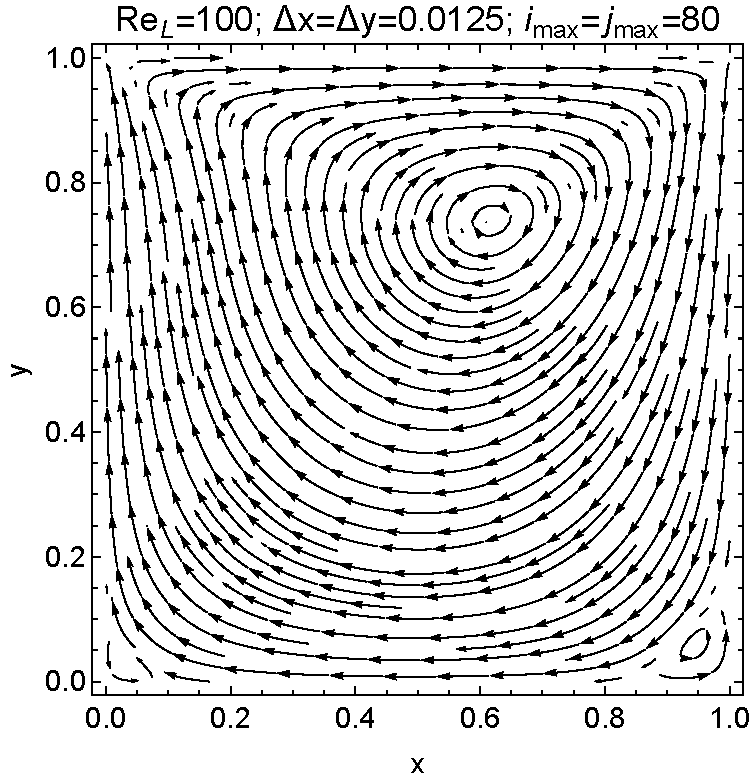
\includegraphics[width=\hsize]{Figures/StreamLines.pdf}
	%\legend{Texto da legenda. (opcional)}
	\source{Citação da fonte ou `O autor' (opcional)}
\end{figure}



Sed ut perspiciatis unde omnis iste natus error sit voluptatem accusantium doloremque laudantium, totam rem aperiam, eaque ipsa quae ab illo inventore veritatis et quasi architecto beatae vitae dicta sunt explicabo. Nemo enim ipsam voluptatem quia voluptas sit aspernatur aut odit aut fugit, sed quia consequuntur magni dolores eos qui ratione voluptatem sequi nesciunt. Neque porro quisquam est, qui dolorem ipsum quia dolor sit amet, consectetur, adipisci velit, sed quia non numquam eius modi tempora incidunt ut labore et dolore magnam aliquam quaerat voluptatem.



Texto da primeira seção. A Figura \ref{rotulo} é o logo da UERJ. 

\begin{figure}[!h]{5cm}
	\caption{Legenda da figura.} \label{rotulo}
	
\includegraphics[width=\hsize]{Figures/logo_uerj_cor.jpg}
	%\legend{Texto da legenda. (opcional)}
	\source{Citação da fonte ou `O autor'. (opcional)}
\end{figure}

Sed ut perspiciatis unde omnis iste natus error sit voluptatem accusantium doloremque laudantium, totam rem aperiam, eaque ipsa quae ab illo inventore veritatis et quasi architecto beatae vitae dicta sunt explicabo. Nemo enim ipsam voluptatem quia voluptas sit aspernatur aut odit aut fugit, sed quia consequuntur magni dolores eos qui ratione voluptatem sequi nesciunt. Neque porro quisquam est, qui dolorem ipsum quia dolor sit amet, consectetur, adipisci velit, sed quia non numquam eius modi tempora incidunt ut labore et dolore magnam aliquam quaerat voluptatem.

Sed ut perspiciatis unde omnis iste natus error sit voluptatem accusantium doloremque laudantium, totam rem aperiam, eaque ipsa quae ab illo inventore veritatis et quasi architecto beatae vitae dicta sunt explicabo. Nemo enim ipsam voluptatem quia voluptas sit aspernatur aut odit aut fugit, sed quia consequuntur magni dolores eos qui ratione voluptatem sequi nesciunt. Neque porro quisquam est, qui dolorem ipsum quia dolor sit amet, consectetur, adipisci velit, sed quia non numquam eius modi tempora incidunt ut labore et dolore magnam aliquam quaerat voluptatem.


Texto da primeira subseção. Figura \ref{outro.rotulo}\subref{subrotulo2}.


\begin{figure}[!h]{8cm}
    \centering
	\caption{Curvas de Nusselt} \label{outro.rotulo}
	\subfloat[][Legenda a...]{\label{subrotulo1}
		\fbox{
\includegraphics[width=0.45\hsize]{Figures/logo_uerj_cinza.png}}}
	\subfloat[][Legenda b...]{\label{subrotulo2}
		\fbox{
\includegraphics[width=0.45\hsize]{Figures/marcadagua_uerj_cinza.png}}}\\
	\subfloat[][Legenda c...]{\label{subrotulo3}
		\fbox{
\includegraphics[width=0.45\hsize]{Figures/logo_uerj_cor.jpg}}}
	\subfloat[][Legenda d...]{\label{subrotulo4}
		\fbox{
\includegraphics[width=0.45\hsize]{Figures/logo_uerj_cinza.png}}}
	%\legend{Texto da legenda (opcional)}
	\source{Citação da fonte ou `O autor'. (opcional)}
\end{figure}


Sed ut perspiciatis unde omnis iste natus error sit voluptatem accusantium doloremque laudantium, totam rem aperiam, eaque ipsa quae ab illo inventore veritatis et quasi architecto beatae vitae dicta sunt explicabo. Nemo enim ipsam voluptatem quia voluptas sit aspernatur aut odit aut fugit, sed quia consequuntur magni dolores eos qui ratione voluptatem sequi nesciunt. Neque porro quisquam est, qui dolorem ipsum quia dolor sit amet, consectetur, adipisci velit, sed quia non numquam eius modi tempora incidunt ut labore et dolore magnam aliquam quaerat voluptatem.


Sed ut perspiciatis unde omnis iste natus error sit voluptatem accusantium doloremque laudantium, totam rem aperiam, eaque ipsa quae ab illo inventore veritatis et quasi architecto beatae vitae dicta sunt explicabo. Nemo enim ipsam voluptatem quia voluptas sit aspernatur aut odit aut fugit, sed quia consequuntur magni dolores eos qui ratione voluptatem sequi nesciunt. Neque porro quisquam est, qui dolorem ipsum quia dolor sit amet, consectetur, adipisci velit, sed quia non numquam eius modi tempora incidunt ut labore et dolore magnam aliquam quaerat voluptatem.


Texto da primeira subsubseção. Tabela \ref{mais.rotulo}.

\begin{table}[!h]{6cm}
	\caption{Título da tabela.}\label{mais.rotulo}
	\centering
	\renewcommand\arraystretch{1.0}
	\begin{tabular}{l|l}
		\hline
		X & Y\\
		\hline
		1,20 & 15,7\\
		1,23 & 15,6\\
		1,19 & 15,3\\
		1,26 & 15,1\\
		1,22 & 15,5\\
		1,16 & 15,3\\
		1,37 & 15,7\\
		\hline
	\end{tabular}
	%\legend{Texto da legenda. (opcional)}
	\source{Citação da fonte ou `O autor'. (opcional)}
\end{table}

Sed ut perspiciatis unde omnis iste natus error sit voluptatem accusantium doloremque laudantium, totam rem aperiam, eaque ipsa quae ab illo inventore veritatis et quasi architecto beatae vitae dicta sunt explicabo. Nemo enim ipsam voluptatem quia voluptas sit aspernatur aut odit aut fugit, sed quia consequuntur magni dolores eos qui ratione voluptatem sequi nesciunt. Neque porro quisquam est, qui dolorem ipsum quia dolor sit amet, consectetur, adipisci velit, sed quia non numquam eius modi tempora incidunt ut labore et dolore magnam aliquam quaerat voluptatem.


Sed ut perspiciatis unde omnis iste natus error sit voluptatem accusantium doloremque laudantium, totam rem aperiam, eaque ipsa quae ab illo inventore veritatis et quasi architecto beatae vitae dicta sunt explicabo. Nemo enim ipsam voluptatem quia voluptas sit aspernatur aut odit aut fugit, sed quia consequuntur magni dolores eos qui ratione voluptatem sequi nesciunt. Neque porro quisquam est, qui dolorem ipsum quia dolor sit amet, consectetur, adipisci velit, sed quia non numquam eius modi tempora incidunt ut labore et dolore magnam aliquam quaerat voluptatem.








\begin{table}[h!]{16cm}
	\caption{Legenda da tabela... \label{tab1}}
	\centering
	%\scriptsize\vspace{-0.5em}
	\renewcommand\arraystretch{1.0}
	\begin{tabular}{|c | c|c|c|c|c|c|c|}
		\hline
		$\xi$ & $\Pe=1$ & $\Pe=2$ & $\Pe=5$ & $\Pe=10$ & $\Pe=20$ & $\Pe=50$ & $\Pe=10^6$  \\
		\hline
		0.01 & 5.22296 & 5.20378 & 5.76517 & 6.51798 & 7.14765 & 7.25370 & 5.97331 \\
		0.02 & 5.22312 & 5.17788 & 5.55262 & 5.94688 & 6.07004 & 5.68785 & 5.01764 \\
		0.03 & 5.22859 & 5.15789 & 5.39565 & 5.56665 & 5.44551 & 5.00668 & 4.63233 \\
		0.04 & 5.23425 & 5.14160 & 5.26962 & 5.28439 & 5.04655 & 4.65836 & 4.43743 \\
		0.05 & 5.24000 & 5.12761 & 5.16310 & 5.06644 & 4.78235 & 4.46566 & 4.33066 \\
		0.1 & 5.26629 & 5.06903 & 4.79158 & 4.50409 & 4.29634 & 4.21132 & 4.19648 \\
		0.2 & 5.28890 & 4.94549 & 4.46973 & 4.26465 & 4.20200 & 4.18899 & 4.18681 \\
		0.3 & 5.27099 & 4.83267 & 4.37396 & 4.23631 & 4.19915 & 4.18883 & 4.18676 \\
		0.4 & 5.22959 & 4.75309 & 4.34476 & 4.23275 & 4.19907 & 4.18883 & 4.18676 \\
		0.5 & 5.18075 & 4.70280 & 4.33558 & 4.23229 & 4.19907 & 4.18883 & 4.18676 \\
		1 & 5.01217 & 4.63313 & 4.33127 & 4.23223 & 4.19907 & 4.18883 & 4.18676 \\
		2 & 4.94867 & 4.62757 & 4.33126 & 4.23223 & 4.19907 & 4.18883 & 4.18676 \\
		5 & 4.94445 & 4.62753 & 4.33126 & 4.23223 & 4.19907 & 4.18883 & 4.18676 \\
		10 & 4.94445 & 4.62753 & 4.33126 & 4.23223 & 4.19907 & 4.18883 & 4.18676 \\
		20 & 4.94445 & 4.62753 & 4.33126 & 4.23223 & 4.19907 & 4.18883 & 4.18676 \\
		50 & 4.94445 & 4.62753 & 4.33126 & 4.23223 & 4.19907 & 4.18883 & 4.18676 \\
		100 & 4.94445 & 4.62753 & 4.33126 & 4.23223 & 4.19907 & 4.18883 & 4.18676 \\
		\hline 
	\end{tabular}
\end{table}



Sed ut perspiciatis unde omnis iste natus error sit voluptatem accusantium doloremque laudantium, totam rem aperiam, eaque ipsa quae ab illo inventore veritatis et quasi architecto beatae vitae dicta sunt explicabo. Nemo enim ipsam voluptatem quia voluptas sit aspernatur aut odit aut fugit, sed quia consequuntur magni dolores eos qui ratione voluptatem sequi nesciunt. Neque porro quisquam est, qui dolorem ipsum quia dolor sit amet, consectetur, adipisci velit, sed quia non numquam eius modi tempora incidunt ut labore et dolore magnam aliquam quaerat voluptatem.



Sed ut perspiciatis unde omnis iste natus error sit voluptatem accusantium doloremque laudantium, totam rem aperiam, eaque ipsa quae ab illo inventore veritatis et quasi architecto beatae vitae dicta sunt explicabo. Nemo enim ipsam voluptatem quia voluptas sit aspernatur aut odit aut fugit, sed quia consequuntur magni dolores eos qui ratione voluptatem sequi nesciunt. Neque porro quisquam est, qui dolorem ipsum quia dolor sit amet, consectetur, adipisci velit, sed quia non numquam eius modi tempora incidunt ut labore et dolore magnam aliquam quaerat voluptatem.

\begin{landscape}
	\begin{figure}[!h]{20cm}
    \centering
	\caption{Exemplo de Página em landscape} \label{outro.rotulo2}
    %\hspace*{-6cm}
	\subfloat[][Legenda a...]{\label{subrotulo5}
		\fbox{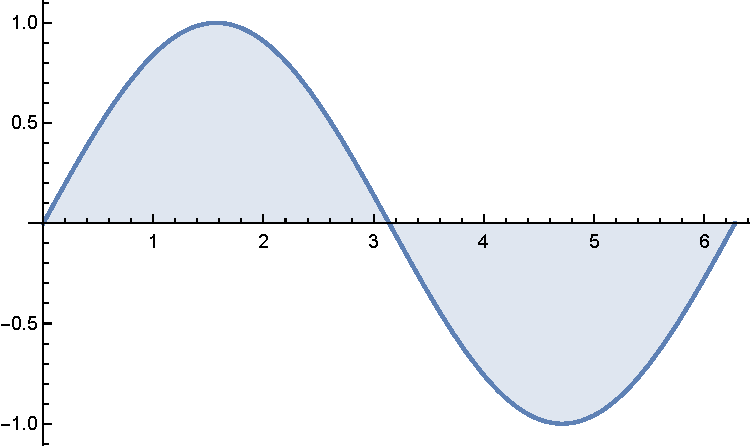
\includegraphics[width=0.5\hsize]{Figures/Plot2.pdf}}}
	\subfloat[][Legenda b...]{\label{subrotulo6}
		\fbox{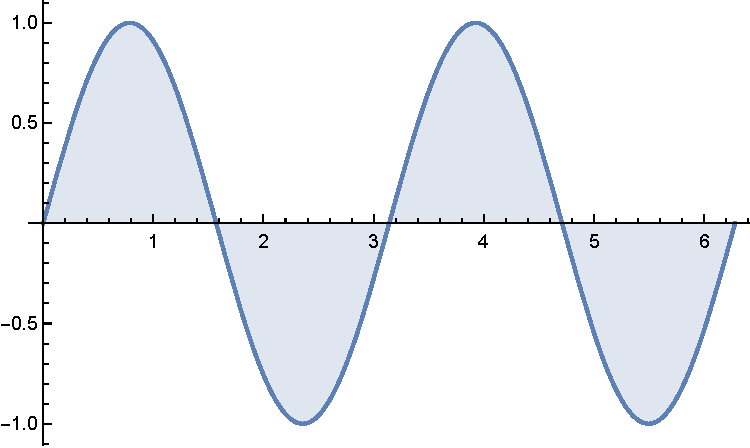
\includegraphics[width=0.5\hsize]{Figures/Plot3.pdf}}}
    \\ %\hspace*{-6cm}
	\subfloat[][Legenda c...]{\label{subrotulo7}
		\fbox{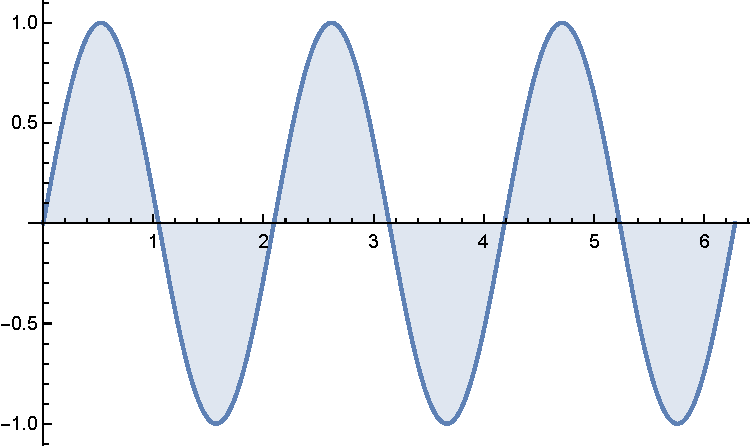
\includegraphics[width=0.5\hsize]{Figures/Plot4.pdf}}}
	\subfloat[][Legenda d...]{\label{subrotulo8}
		\fbox{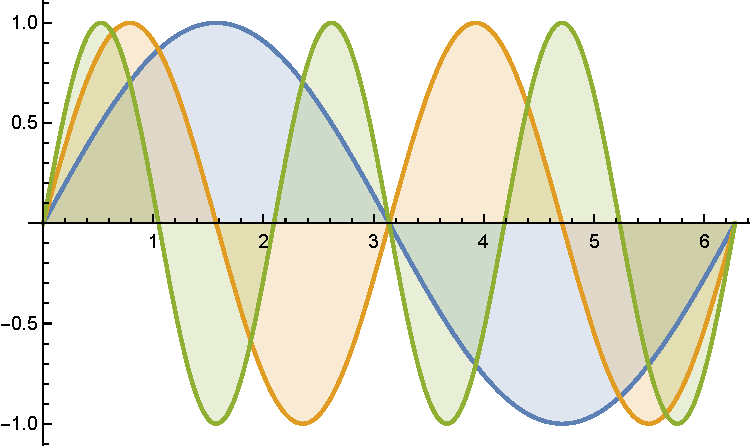
\includegraphics[width=0.5\hsize]{Figures/Plot1.pdf}}}
	%\legend{Texto da legenda (opcional)}
	\source{Citação da fonte ou `O autor'. (opcional)}
	\end{figure}
\end{landscape}








%=====================================================================
\chapter*{Conclusão}
%=====================================================================

Lorem ipsum dolor sit amet, consectetur adipiscing elit, sed do eiusmod tempor incididunt ut labore et dolore magna aliqua. Ut enim ad minim veniam, quis nostrud exercitation ullamco laboris nisi ut aliquip ex ea commodo consequat. Duis aute irure dolor in reprehenderit in voluptate velit esse cillum dolore eu fugiat nulla pariatur. Excepteur sint occaecat cupidatat non proident, sunt in culpa qui officia deserunt mollit anim id est laborum.

Lorem ipsum dolor sit amet, consectetur adipiscing elit, sed do eiusmod tempor incididunt ut labore et dolore magna aliqua. Ut enim ad minim veniam, quis nostrud exercitation ullamco laboris nisi ut aliquip ex ea commodo consequat. Duis aute irure dolor in reprehenderit in voluptate velit esse cillum dolore eu fugiat nulla pariatur. Excepteur sint occaecat cupidatat non proident, sunt in culpa qui officia deserunt mollit anim id est laborum.

Lorem ipsum dolor sit amet, consectetur adipiscing elit, sed do eiusmod tempor incididunt ut labore et dolore magna aliqua. Ut enim ad minim veniam, quis nostrud exercitation ullamco laboris nisi ut aliquip ex ea commodo consequat. Duis aute irure dolor in reprehenderit in voluptate velit esse cillum dolore eu fugiat nulla pariatur. Excepteur sint occaecat cupidatat non proident, sunt in culpa qui officia deserunt mollit anim id est laborum.

Lorem ipsum dolor sit amet, consectetur adipiscing elit, sed do eiusmod tempor incididunt ut labore et dolore magna aliqua. Ut enim ad minim veniam, quis nostrud exercitation ullamco laboris nisi ut aliquip ex ea commodo consequat. Duis aute irure dolor in reprehenderit in voluptate velit esse cillum dolore eu fugiat nulla pariatur. Excepteur sint occaecat cupidatat non proident, sunt in culpa qui officia deserunt mollit anim id est laborum.

Lorem ipsum dolor sit amet, consectetur adipiscing elit, sed do eiusmod tempor incididunt ut labore et dolore magna aliqua. Ut enim ad minim veniam, quis nostrud exercitation ullamco laboris nisi ut aliquip ex ea commodo consequat. Duis aute irure dolor in reprehenderit in voluptate velit esse cillum dolore eu fugiat nulla pariatur. Excepteur sint occaecat cupidatat non proident, sunt in culpa qui officia deserunt mollit anim id est laborum.















% ----------------------------------------------------------
%% ELEMENTOS POS-TEXTUAIS
% ----------------------------------------------------------
\backmatter
%=====================================================================
% Referencias via BibTeX
%=====================================================================
\citeoption{abnt-options4}
\bibliography{A.Bibliography/MyBibliography}
%=====================================================================




%=====================================================================
%% Glossário
%=====================================================================
%=====================================================================
\postextualchapter*{Glossário}
%=====================================================================


\definicao{termo 1}{significado}
\definicao{termo 2}{significado}
\definicao{termo 3}{significado}




% ----------------------------------------------------------
% Apêndices (opcionais)
% ----------------------------------------------------------
% ---
% Inicia os apêndices
% ---
\appendix

%=====================================================================
\postextualchapter{Primeiro apêndice}
%=====================================================================
\section{Primeira seção}

Texto da primeira seção\index{Introdução!Capítulo}.

\subsection{Primeira subseção}

Texto da primeira subseção.

\subsubsection{Primeira subsubseção}

Texto da primeira subsubseção.

%=====================================================================
\postextualchapter{Segundo apêndice}
%=====================================================================
\section{Primeira seção}

Texto da primeira seção.

\subsection{Primeira subseção}

Texto da primeira subseção.

\subsubsection{Primeira subsubseção}

Texto da primeira subsubseção.






% ----------------------------------------------------------
% Anexos (opcionais)
% ----------------------------------------------------------
% ---
% Inicia os anexos
% ---
\annex

%=====================================================================
\postextualchapter{Primeiro anexo}
%=====================================================================

Modelo de trabalho acadêmico utilizando classe repUERJ para elaboração de teses, dissertação e monografias em geral (projetos finais e trabalhos de conclusão de curso).

Este modelo foi criado por Dr. Luís Fernando de Oliveira, Professor Adjunto do Departamento de Física Aplicada e Termodinâmica, Instituto de Física Armando Dias Tavares da Universidade do Estado do Rio de Janeiro -- UERJ

A classe repUERJ.cls foi criada a partir do código original disponibilizado pelo grupo CódigoLivre.Org (equipe coordenada por Gerald Weber). Foram feitas adequações para implementação das normas de elaboração de teses e dissertações da UERJ.

Os estilos repUERJformat.sty codificam os elementos pré-textuais e pós-textuais.

O estilo repUERJpseudocode.sty codifica a elaboração de algoritmos utilizando um glossário desenvolvido por mim (Luís Fernando), o mesmo usado em meu curso de Física Computacional.

Este arquivo está editado na codificação de caracteres UTF-8.

As referencia estão baseadas no modelo bibtex e citação em autor-data.

Todo este material está disponível também no meu site \url{http://sites.google.com/site/deoliveiralf}.

As normas da UERJ para elaboração de teses e dissertações pode ser obtidas no documento disponível no site \url{http://www.bdtd.uerj.br/roteiro_uerj_web.pdf}.

Agradecimentos ao NPROTEC/Rede Sirius/UERJ e à Biblioteca Setorial da Física.


%=====================================================================
\postextualchapter{Segundo anexo}
%=====================================================================
\section{Primeira seção}

Texto da primeira seção.

\subsection{Primeira subseção}

Texto da primeira subseção.

\subsubsection{Primeira subsubseção}

Texto da primeira subsubseção.



%---------------------------------------------------------------------
%% INDICE REMISSIVO (relativo ao makeindex)
%---------------------------------------------------------------------
\printindex
%=====================================================================
\end{document}
